\chapter{Radomes}

\section{Introduction to Radomes}

A radome (short for “radar dome”) is an electromagnetic enclosure that protects antennas from environmental factors such as wind, rain, dust, temperature fluctuations, and physical damage. While offering mechanical protection, a well-designed radome must remain electromagnetically transparent, ensuring minimal degradation of antenna performance in terms of gain, beam shape, or impedance matching.

Radomes are especially critical in radar, aerospace, and radio astronomy systems, where precise radiation characteristics and consistent long-term operation are required. Improperly chosen radome parameters can lead to signal attenuation, beam distortion, and multipath reflections.

\section{Material Considerations}

An ideal radome material exhibits the following characteristics:

\begin{itemize}
    \item Low relative permittivity ($\varepsilon_r$) — reduces phase delay and impedance mismatch
    \item Low dielectric loss tangent ($\tan\delta$) — minimizes absorption
    \item High mechanical durability and environmental resistance
    \item Stable performance over temperature and frequency variations
\end{itemize}

Common radome materials include PTFE (Teflon), ABS, polycarbonate, and PMMA (Plexiglass). The material used in this study is PMMA, with $\varepsilon_r = 2.8$ and $\tan\delta = 0.001$ at 6~GHz.

\section{Electromagnetic Theory of Radomes}

\subsection*{i. Transmitted and Reflected Wave Behavior}

When an EM wave encounters a dielectric slab (the radome wall), it experiences partial transmission and reflection. The reflection coefficient $\Gamma$ at the air–radome interface is given by:

\[
\Gamma = \frac{\sqrt{\varepsilon_r} - 1}{\sqrt{\varepsilon_r} + 1}
\]

The transmitted wave continues through the radome material with a different wavelength, experiencing phase shift. Multiple reflections inside the slab can constructively or destructively interfere depending on thickness and incident angle.

To minimize reflections and phase distortion, **transmission line analogy** is used. The dielectric slab acts like a transmission line segment of impedance $Z_m = \frac{Z_0}{\sqrt{\varepsilon_r}}$, where $Z_0$ is the impedance of free space.

\subsection*{ii. Optimal Distance Between Antenna and Radome}

The separation between the antenna and radome wall should be carefully selected to prevent standing wave formation and phase errors caused by internal reflections. An optimal distance $D$ satisfies the condition:

\[
D_{\text{opt}} = n \cdot \frac{\lambda_0}{2}, \quad n \in \mathbb{Z}^+
\]

where $\lambda_0$ is the free-space wavelength. At these distances, reflected waves from the radome re-enter the antenna in-phase, minimizing destructive interference.

\subsection*{iii. Optimal Radome Wall Thickness}

To minimize reflections at the radome wall, the thickness $t$ should satisfy the **half-wave matching condition** in the radome material:

\[
t_{\text{opt}} = n \cdot \frac{\lambda_0}{2\sqrt{\varepsilon_r}}, \quad n \in \mathbb{Z}^+
\]

This ensures that reflected waves inside the radome destructively interfere, reducing the effective reflection seen by the antenna. For instance, at 6~GHz and $\varepsilon_r = 2.8$, $\lambda_0 = 50~\mathrm{mm}$, leading to an optimal thickness of approximately:

\[
t \approx \frac{50}{2 \cdot \sqrt{2.8}} \approx 14.95~\mathrm{mm}
\]

for $n = 1$.

\subsection*{iv. Errors Introduced by Flat Radomes}

Flat radomes are simple to manufacture but introduce angular-dependent errors due to refraction and differential phase delay. Key error sources include:

\begin{itemize}
    \item \textbf{Beam broadening or squinting}: Radiation pattern shifts due to phase mismatch.
    \item \textbf{Ripple in gain pattern}: Standing waves between antenna and inner wall.
    \item \textbf{Side lobe distortion}: Especially for wider beams or off-axis rays.
    \item \textbf{Frequency sensitivity}: Optimal thickness and spacing vary with frequency.
\end{itemize}

These errors worsen at large incidence angles and are minimized by curvature-matched (e.g., spherical or conical) radomes in high-precision applications.

\begin{figure}[H]
    \centering
    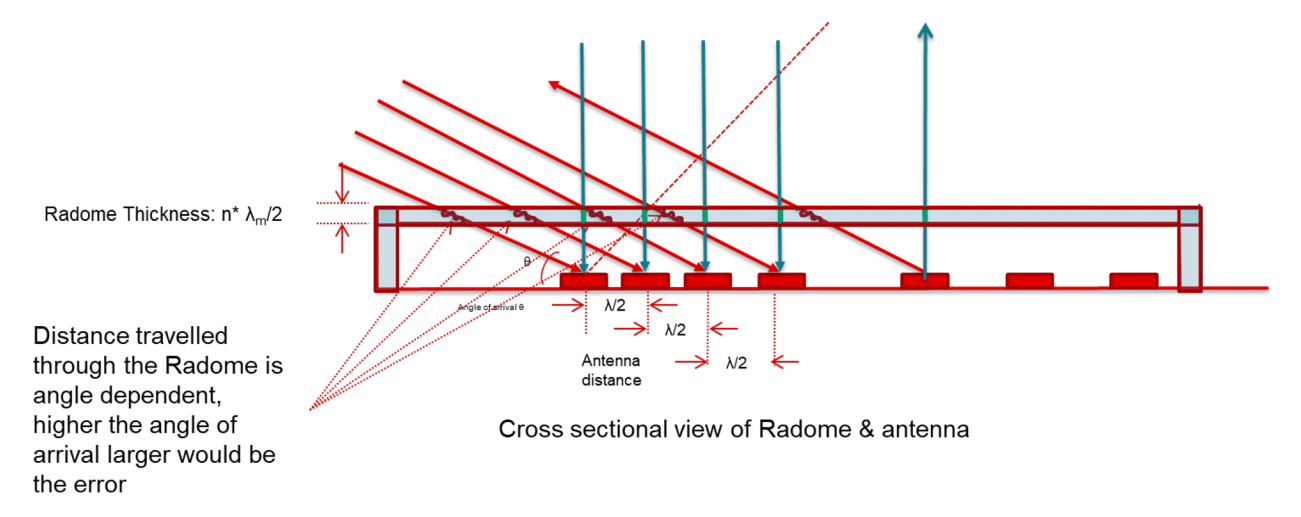
\includegraphics[width=0.9\textwidth]{figures/flat.png}
    \caption{Distance Traveled in Rectangular Radome Wall for Different Grazing Angles.}
    \small Image adapted from \cite{swra705}.
    \label{fig:radome-grazing-angle}
\end{figure}

\section{Design Summary}

To ensure optimal performance:

\begin{itemize}
    \item Select low-loss, low-permittivity materials (e.g., PMMA, PTFE)
    \item Match radome thickness to a multiple of half-wavelength in the material
    \item Set antenna-to-radome spacing to avoid phase error from internal reflections
    \item Consider the operating frequency range and beamwidth in the design
\end{itemize}

These considerations enable the radome to function as a passive, protective structure without compromising the electromagnetic integrity of the antenna system.

\section*{Conclusion}

This chapter explored the function, design parameters, and electromagnetic impact of radomes. Key derivations included reflection coefficients, optimal wall thickness, and antenna-to-radome spacing. Flat radomes, while practical, were shown to introduce beam distortion and phase errors if improperly designed. These theoretical insights will now be applied in the following chapter, where we focus on modeling the microstrip patch antenna to be enclosed by such radomes.
